%%%%%%%%%%%%%%%%%%%%%%%%%%%%%%%%%%%%%%%%%%%%%%%%%%%%%%%%
%%%%%%%%%%%%%%%%%%%%%%%%%%%%%%%%%%%%%%%%%%%%%%%%%%%%%%%%
\section{Discussion}
\label{sec:discussion}
%%%%%%%%%%%%%%%%%%%%%%%%%%%%%%%%%%%%%%%%%%%%%%%%%%%%%%%%
%%%%%%%%%%%%%%%%%%%%%%%%%%%%%%%%%%%%%%%%%%%%%%%%%%%%%%%%
%
Overall, we note a positive relationship between FIM skill and a reduction of the stream order of the stream network we use to derive the HAND datasets.
Most of this change is accounted for by increasing POD thus reducing FNs especially along higher order rivers with higher flow magnitudes.
We note that reducing stream order does in turn suffer from diminishing returns in which the increase in mapping skill for applying stream order reduction to roughly 4-5\% of the stream network is about the same as the increase for applying stream order reduction to the remaining 95-96\% of the stream network.
This motivates further work in identifying what the optimal coverage of stream order reduction could be and how to parameterize that coverage. 
One option could be removing stream orders ones and possibly twos and threes from stream order reduction and simply using the inundation from FR from these areas.

In analyzing the data, we found a slight reduction in FAR was detected and more digging pointed to a bias in rating curves introduced by stream order reduction.
Figure \ref{fig:rating_curve_comparison} illustrates the general effect that stream order reduction has on synthetic rating curves.
Sub-figure \ref{fig:rating_curve_comparison}a shows how the average rating curves for all reaches for stage values 0 to 25 meters at one-third meter intervals tend to bias down (and to the right) with ever increasing stream order reduction (FR to MS to GMS). 
This bias is more pronounced for GMS since that implements stream order reduction down to the unit level for the entire FR network while MS only does so for 4-5\% of the network.
Attempting to diagnose this bias in the SRC leads one to Equation \ref{eq:reach_averaged_mannings_equation} which shows the reach averaged synthetic rating curve relationship between stage and discharge.
Across the three methods explored, FR, MS, and GMS, one identifies differences in the inputs and outputs and notes no difference in the stages and Manning's n values.
While the channel slope and reach lengths are not exactly the same across methods, their averaged differences are very negligible which only leaves room for deviations in volume and bed area.
Again, volume (V[y] or simply V) is synonymous to reach-averaged cross-sectional area and bed area (B[y] or B) is analogous to reach-averaged hydraulic radius.
Discharge, Q, is directly related to volume and inversely related to bed area and each parameter is weighed according to the magnitude of its exponent which are $\frac{5}{3}$ and $\frac{2}{3}$ respectively. 
Figures \ref{fig:rating_curve_comparison} b and c show how volume and bed area compare across the three methods with GMS having significantly greater values than MS which has greater values than FR.
Again the relative discrepancy between FR vs MS and MS vs GMS is explained by the extent of their spatial coverages.
Both V and B values increase but since both are weighed differently by their respective exponents and pull Q in different directions.
We show in Figure \ref{fig:rating_curve_comparison}d the relationship of $\frac{V^{5/3}}{B^{2/3}}$ is plotted against stage, y, to show how these two parameters collectively pull the rating curve Q up and biases the rating curve down.
In other words, the magnitude and weight of the volume at each stage level exceeds the influence of the magnitude and weight of the bed area.
Both parameters are set to increase mainly due to much larger catchments leading to more pixels at each stage level as shown in Figure \ref{fig:rating_curve_comparison}e.
Much of the increase in inundated pixels, volume, and bed area can be explained by much larger catchments that encompass neighboring tributaries.
These tributaries have a significant amount of bathymetry that is low-lying thus easily including the SRC derivation. 
They also contribute volume and bed area that is technically not perpendicular to the flux of streamflow being accounted for in the stream in question. 
Careful examination of Figure \ref{fig:gms_enhancement}b shows how much larger catchments include neighboring tributaries and the geometry associated with those tributaries. 
This geometry is not perpendicular to the flow that is associated with the main reach thus leading to biases in the SRC.
We consider this fact to have a nuanced effect on skill, while reducing the rate of FPs it also can lead to FNs due to biases in the SRC.

Additional careful analysis of Figure \ref{fig:gms_enhancement}a, leads one to note many catchments that don't have inundation or significant inundation.
While the cause of these errors can be varied, we assert here that conflating 4 networks for use in evaluations leads to significant error.
As one may remember, Section \ref{sssec:cross_walking_networks} details how reach identifiers are conflated for the FIM network back to that of the NWM. 
One of the issues is when a reach of given stream order accidentally conflates to that of a neighboring tributary that is of lower order which leads to areas of FNs.
The utilization of MS and GMS only conflates to NWM catchments directly associated with the level path in question which is inherently easy to do with those methods. 
Thus part of the improvement in MS and GMS methods is due to a slight improvement in cross-walking methodology.
The NWM stream network was derived using the NHD medium resolution dataset which was derived from coarser DEMs than those used here. 
Additional conflation is identified in cross-walking the stream network used by the BLE maps and those of HAND.
Until a singular stream network is used for the NWM, BLE benchmark, and for HAND based FIM, conflation will continue being a source of error.

Our qualitative analysis suggests that the synthetic rating curves offer a significant opportunity for improvement in HAND based FIM for future development.
The bathymetry of the NED 10m DEM is known to be lacking proper representation thus leading to inadequate representation of volume and bed area with all three methods employed.
Manning's n which typically accounts for roughness could be tuned to account for these DEM limitations or could be held fixed to some local value associated with a given flood magnitude.
Some adjusting parameter must be introduced to enhance the estimation of the bathymetric representation.
Lidar DEMs from the USGS at 3m and 1m scale could be utilized to derive HAND as well which we conject should show better agreement with higher fidelity FIMs also derived from the same Lidar based DEMs.

Lastly, after errors introduced by conflation, poor roughness estimation, bathymetric/elevation adjustment are accounted for, HAND still has another fundamental limitation that is inherently baked into how it works.
For HAND to be derived and thus create a FIM for a given area, that area must entirely drain to the stream network and the stream network must also drain itself.
In other words, an entire area eligible for flooding must monotonically decrease in elevation. 
DEM's naturally don't do this and the dynamics of true flood events don't follow drainage patterns.
Enforcing this assumption for HAND leads to significant amount of DEM manipulations that introduce basic errors.
These errors are deep into the assumptions of HAND and thus more difficult to disentangle.
Ultimately, the use of more advanced 2-D hydrodynamic models should be considered for dealing with this limitation of HAND but would come at significant expense at the given high resolution across very large spatial scales and frequent forecast resolutions.
%
\begin{figure}[h!]
\centering
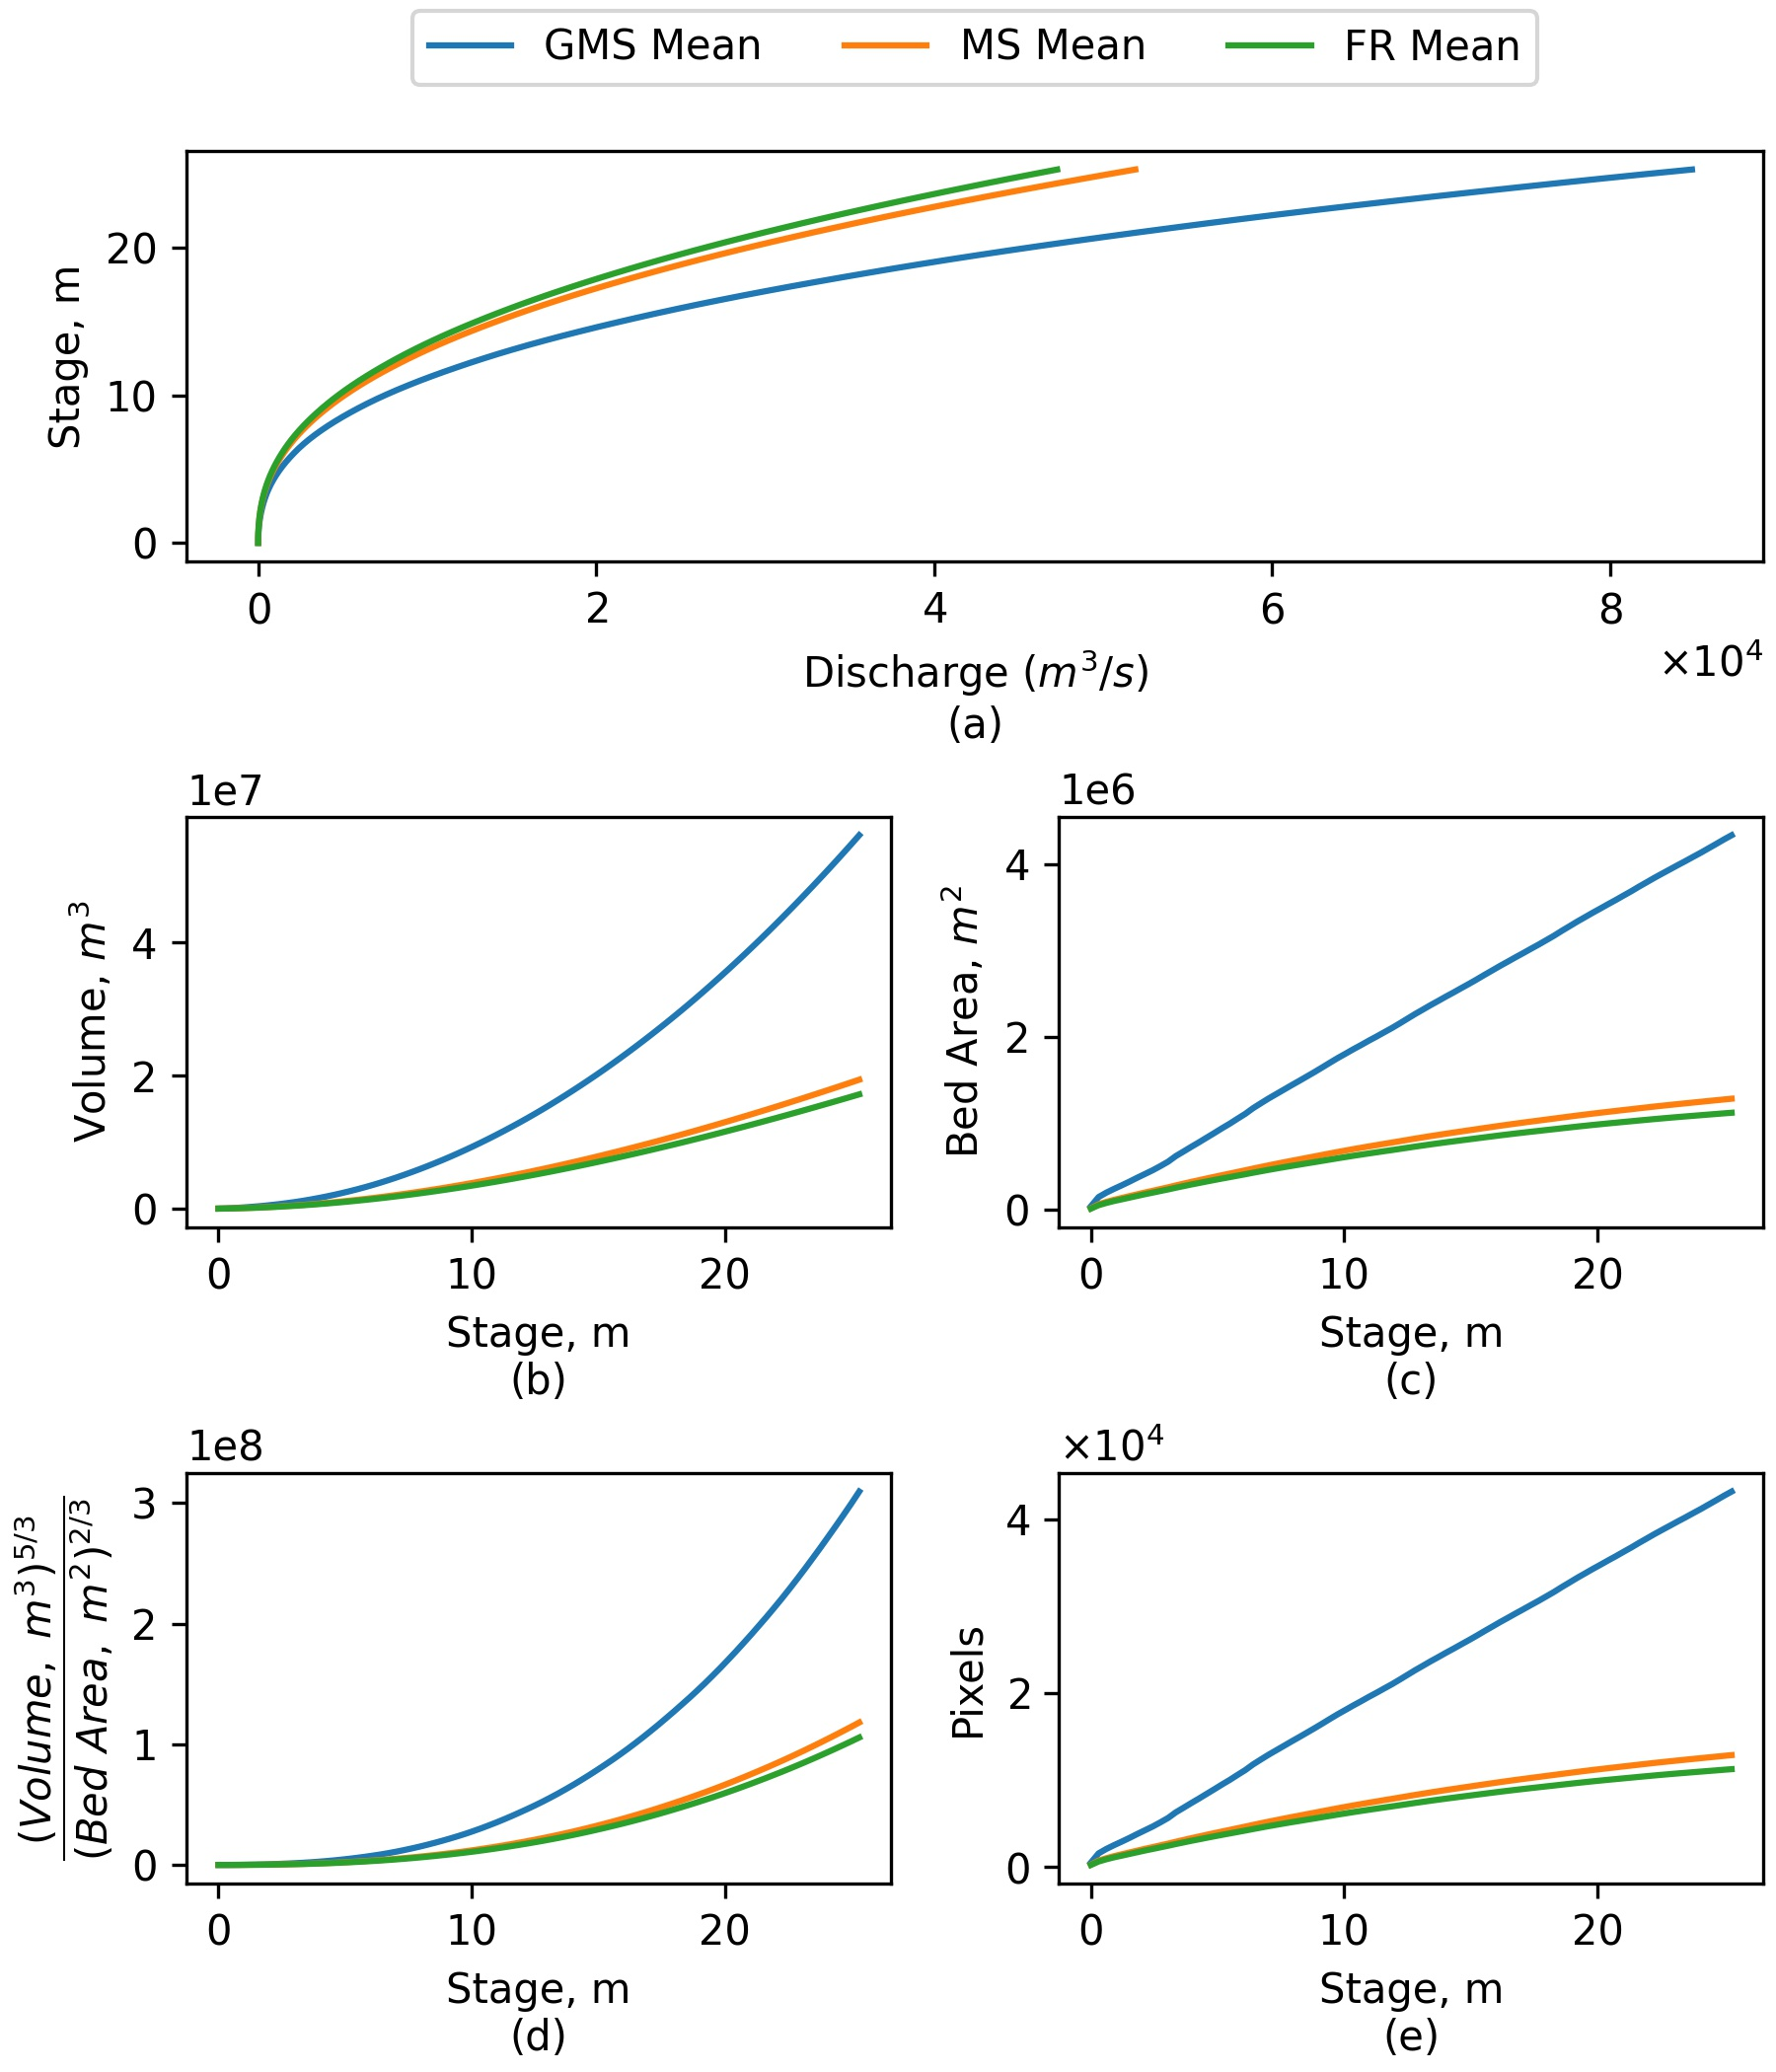
\includegraphics[scale=1.0]{figures/rating_curve_comparison.jpg}
\caption{Illustrates average quantities for the three methods, FR, MS, and GMS, for each stage value (m). 
The values are (a) Discharge $m^3s^{-1}$, (b) Volume $m^3$, (c) Bed Area $m^2$, (d) a function of Volume and Bed Area, and (e) number of pixels.
}
\label{fig:rating_curve_comparison}
\end{figure}
%
%
\begin{figure}[h!]
\centering
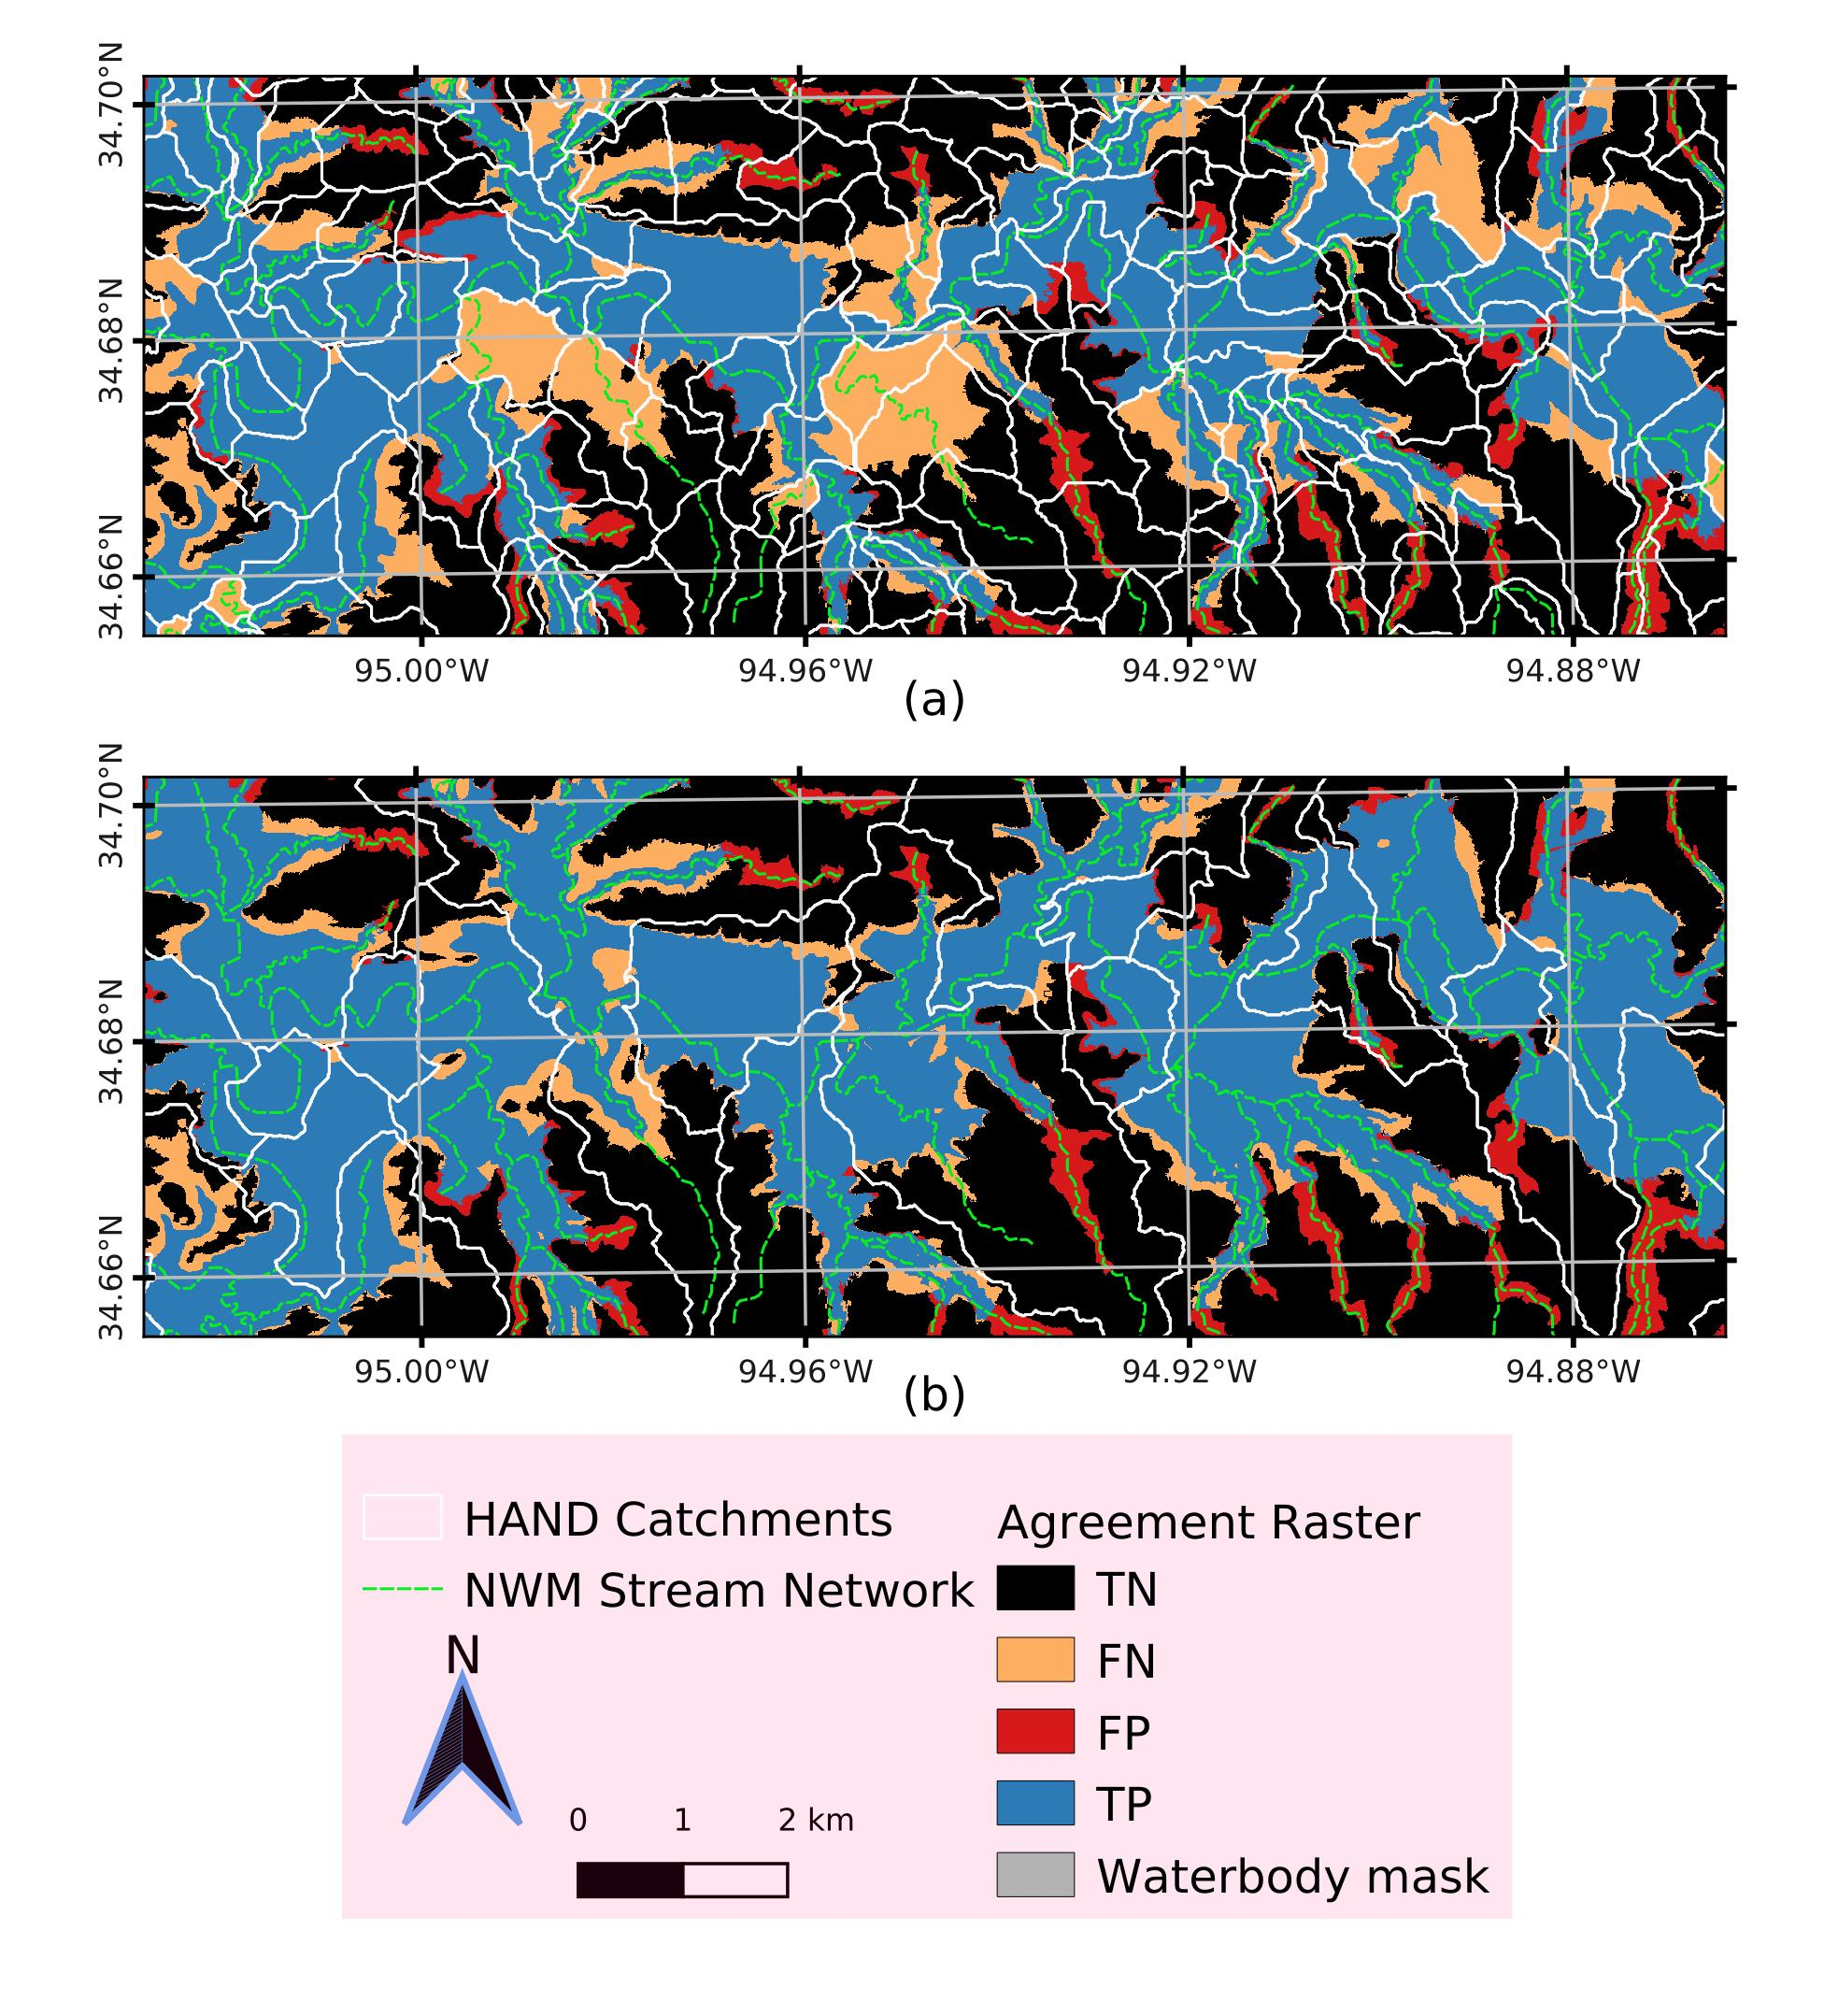
\includegraphics[scale=1.0]{figures/gms_enhancement.jpg}
\caption{OWP FIM `Cahaba' inundation agreement, TP, FP, FN, and TN, with BLE HEC-RAS maps in HUC 11140105.
Catchment boundaries and stream lines are shown in white and dotted green, respectively.
Sub-figure (a) shows agreement of FR HAND denoting significant areas of under-prediction due to junctions and catchment boundaries.
Meanwhile, (b) shows the agreement for GMS and much larger catchments leading to much better inundation agreement for this given reach. 
Overall, this illustrates the benefits of stream order reduction for deriving HAND datasets.
}
\label{fig:gms_enhancement}
\end{figure}
%
